%!TEX root = hard_stack_paper/paper.tex

\begin{figure*}[t]
\begin{subfigure}[t]{\textwidth}
\centering
\scalebox{0.8}{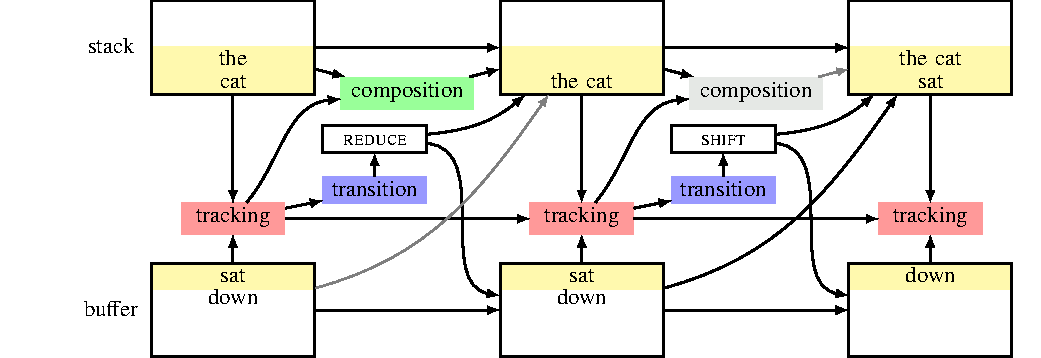
\includegraphics{CompiledTikzPictures/paper-figure2.pdf}}
  
 \caption{The SPINN model unrolled for two transitions during the processing of the sentence \word{the cat sat down}. `Tracking', `transition', and `composition' are neural network layers. Gray arrows indicate connections which are blocked by a gating function.}\label{fig:model:1d}
  
\end{subfigure}\\\\\\
\begin{subfigure}[t]{\textwidth}
\centering
\scalebox{0.5}{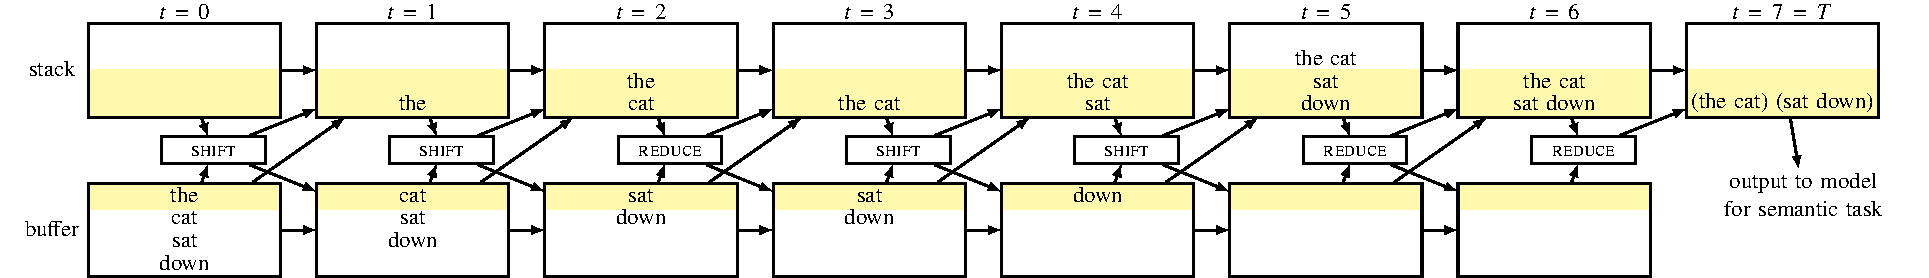
\includegraphics{CompiledTikzPictures/paper-figure3.pdf}}
  
 \caption{The fully unrolled SPINN for \word{the cat sat down}, with neural network layers omitted for clarity.}\label{fig:model:1b}  
\end{subfigure}
\caption{\label{fig:m1-views}Two views of the Stack-augmented Parser-Interpreter Neural Network (SPINN).}
\end{figure*}
